\subsection{Circuito RC}\label{sec: RC}
\paragraph{}
En esta sección, se estudió la repuesta de un circuito RC en su régimen transitorio. El circuito montado se observa en la figura \ref{esq: RC}, donde se conectaron en serie un resistor de resistencia variable y un capacitor de capacidad $C=\SI{9.39(0.07)e-9}{F}$. El sistema se alimentó con una fuente de ondas cuadradas de tensión $V_0=\SI{10.4(0.5)}{V}$. 
\paragraph{}
Se registró la caída de tensión en la resistencia a partir del osciloscopio, obteniéndose la tensión en función del tiempo. Se realizó un barrido de resistencias de $\SI{1000(9)}{\Omega}$ hasta $\SI{10.0(0.2)e6}{\Omega}$, capturando los datos del osciloscopio en cada caso y se hizo un ajuste por medio de la ecuación \eqref{eqn:RC} para calcular $\tau_1$. Un ejemplo de este ajuste se observa en la figura \ref{fig:RC barrido}, donde $R=\SI{316.2(0.6)e4}{\Omega}$.
\begin{figure} [H]
    \centering
    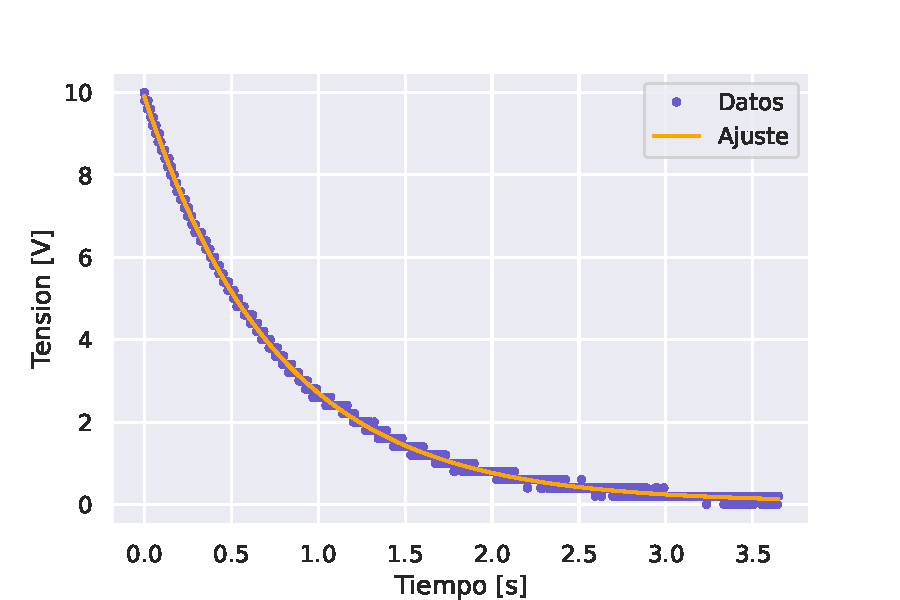
\includegraphics[scale=0.7]{Figuras/RC/RC 3162000.pdf}
    \caption{Gráfico de la tensión en función del tiempo para $R=\SI{316.2(0.6)e4}{\Omega}$ y su ajuste. Los residuos presentan una distribución aparentemente aleatoria.}
    \label{fig:RC barrido}
\end{figure}
\paragraph{}
Del ajuste de la figura \ref{fig:RC barrido}, se puede obtener el correspondiente valor de $\tau_1=\SI{1.311(0.003)}{s}$ y, con la ecuación \eqref{eqn:tau 1}, el valor de $C$. Para este valor de resistencia, $C=\SI{4.1(0.2)e-7}{F}$, lo cual presenta diferencias significativas con la capacidad medida independientemente. No se considera que haya otra capacidad que no se esté considerando, ya que la diferencia es de dos órdenes de magnitud.
\paragraph{}
Los valores de $\tau_1$ obtenidos del barrido de resistencias fueron analizados mediante la ecuación \eqref{eqn:tau 1}, donde $\tau_1$ tiene una relación lineal con $R$, y la pendiente de dicha función lineal es $C$. Como muestra la figura \ref{fig:RC tau}, esta relación no es lineal.
\begin{figure} [H]
    \centering
    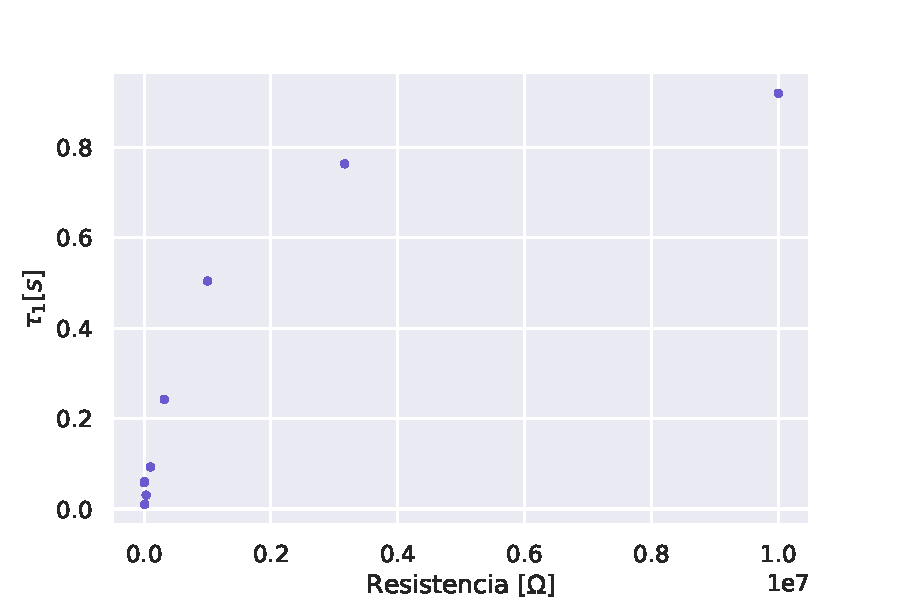
\includegraphics[scale=0.7]{Figuras/RC/rc_tau.pdf}
    \caption{Gráfico de $\tau_1$ en función de $R$. Los puntos no tienen una distribución lineal, lo cual no concuerda con el modelo dado por la ecuación \eqref{eqn:tau 1}.}
    \label{fig:RC tau}
\end{figure}
\paragraph{}
Los valores de $\tau_1$ obtenidos de cada ajuste no presentan una distribución lineal, es decir, no siguen el modelo dado por \eqref{eqn:tau 1}. Esto, junto con las diferencias significativas que se encontraron entre los valores de $C$, lleva a la conclusión de que existen parámetros relevantes que no fueron considerados a la hora de armar el circuito. Un candidato posible es la impedancia del equipo de medición la cual es de un orden semejante a la de los componentes y por lo tanto difícilmente ignoranles. Sin embargo no podemos concluir nada sobre esta relación ni sobre el modelo.